\documentclass[12pt, a4paper]{report}
\usepackage[square, numbers, comma, sort&compress]{natbib} 
\usepackage[utf8]{inputenc}
\usepackage{graphicx}
\graphicspath{ {media/} }
\usepackage{hyperref}
\usepackage{fancyhdr}
\usepackage{listings}
\usepackage{cleveref}
\usepackage{xcolor}
\renewcommand{\lstlistingname}{Code}
\renewcommand{\lstlistlistingname}{List of Code}

\lstdefinestyle{chstyle}{%
backgroundcolor=\color{gray!12},
basicstyle=\ttfamily\small,
commentstyle=\color{green!60!black},
keywordstyle=\color{magenta},
stringstyle=\color{blue!50!red},
showstringspaces=false,
%captionpos=b,
numbers=left,
numberstyle=\footnotesize\color{gray},
numbersep=10pt,
%stepnumber=2,
tabsize=2,
frame=L,
framerule=1pt,
rulecolor=\color{red},
breaklines=true,
inputpath=code
}
\usepackage[legalpaper, leftmargin=0.8in]{geometry}
\pagestyle{fancy}
\lhead{Team-5}
\rhead{\empty}
\rfoot{Page \thepage}


\begin{document}

\begin{titlepage}


    
    \begin{center}

      \uppercase{{\LARGE \bf Report \par}}
 {\LARGE \bf on \par}
      \smallskip
      { \Large \bf \em ``Network Sniffing with Wireshark Similar Tool'' \par}
     {\Large \bf Course: ``Computer Security'' \linebreak}

      %{\large in \par}
      
      

       
\includegraphics[width=5cm]{image5.png}\par 

       {\Large \bf Course Code: CS4035D\par}
       {\large \bf Department of Computer Science and Engineering,\par}
       {\large \bf National Institute of Technology, Calicut \par}
       {\large \bf Calicut, Kerala, India – 673 601 \par}
       

    \end{center}
    
    
        {\Large \em Submitted by }
        \hfill
        {\Large \em Submitted to \\} 
        \smallskip
        {\large \bf Dr. Vasudevan, A. R. }
        \hfill
        {\large \bf Abhijeet kumar singh \\}
        {\large \bf Department of CSED }
        \hfill
        {\large \bf M190675CA\\}
        \null\hfill
        { \large \bf Ashish Kumar Sahu\\}
        \null\hfill
        {\large \bf  M190365CA\\}
        \null\hfill
	    { \large \bf Abhilasha Sharma\\}
	    \null\hfill
        {\large \bf  M180275CA\\}

    

  \end{titlepage}





\chapter{Network Sniffing Using Wireshark}

\section{\emph{Introduction}}

\subsection{What is Sniffing}

Sniffing can be defined as a process that refers to investigating
something covertly in order to find any confidential information. By an
information security perspective, sniffing refers to tapping the traffic
or routing the traffic to a target where it can be captured, analyzed
and monitored. It is mostly performed to analyze the usage of network,
troubleshooting any network issues, session monitoring for development
and the testing purposes.

The network packets or TCP/IP packet contains vital information which is
required for two network interfaces to communicate with each other. It
contains fields that are source and destination IP addresses, ports,
sequence numbers and the protocol type. All of these fields are crucial
for various network layers to function properly, and especially for the
Layer 7 application which makes use of the received data.

\subsection{What is Packet Sniffing}

The data that has to be transmitted over the computer network, is
firstly and foremost broken down into smaller units at the sender's node
called \emph{data packets} and at the receiver's node it is resembled in
original format. So we can say that it is the \emph{smallest unit} of
communication over a computer network. These packets are also called a
block, a segment, a cell or a datagram. Capturing these data packets
when it is flowing from one device to another over a network is known as
\textbf{packet sniffing}. We can assume that it is similar to
wiretapping to a telephone network.These are mostly used by
\emph{crackers and hackers} to collect information illegally from the
network. \emph{ISPs, advertisers and governments also use such softwares
to capture packets}.

\subsection{What is Wireshark}

Wireshark is one of the best network packet analyzer, which is an
essential tool for security professionals and system administrators. It
is a free and open source packet analyzer, the purpose of this packet
analyzer is to present captured packet data in as much detail as
possible.

We can think that network packet analyzer is like a measuring device for
examining what's happening inside a network cable,which is similar to an
electrician that uses a voltmeter for examining what's happening inside
an electric cable.It is a tool that intercepts traffic and converts that
binary traffic into human-readable format, which makes it easy to
identify what type of traffic is crossing your network, how much of it,
how frequently it transfers, the latency there is between certain hops,
and so forth.

\subsection{\Large \emph{References: }}
\begin{flushleft}
\href{https://www.greycampus.com/blog/information-security/what-is-a-sniffing-attack-and-how-can-you-defend\%20it\#:~:text=From\%20an\%20information\%20security\%20perspective,for\%20development\%20and\%20testing\%20purpose.}{https://www.greycampus.com/blog/information-security/what-is-a-sniffing-attack-and-how-can-you-defend\%20it\#:~:text=From\%20an\%20information \ \%20security\%20perspective,for\%20development\%20and\%20testing \ \%20purpose.}
\bigbreak
\href{https://www.valencynetworks.com/articles/cyber-security-attacks-network-sniffing.html}{\emph{https://www.valencynetworks.com/articles/cyber-security-attacks-network-sniffing.html}}
\bigbreak
\href{https://www.geeksforgeeks.org/what-is-packet-sniffing/}{\emph{https://www.geeksforgeeks.org/what-is-packet-sniffing/}}
\bigbreak
\href{https://www.csoonline.com/article/3305805/what-is-wireshark-what-this-essential-troubleshooting-tool-does-and-how-to-use-it.html}{\emph{https://www.csoonline.com/article/3305805/what-is-wireshark-what-this-essential-troubleshooting-tool-does-and-how-to-use-it.html}}
\end{flushleft}
\chapter{\emph{Working of wireshark}}

\begin{enumerate}
\def\labelenumi{\arabic{enumi})}
\item
  After successful installation of wireshark, launch the application.
  The interface of the application would be like
  \begin{center}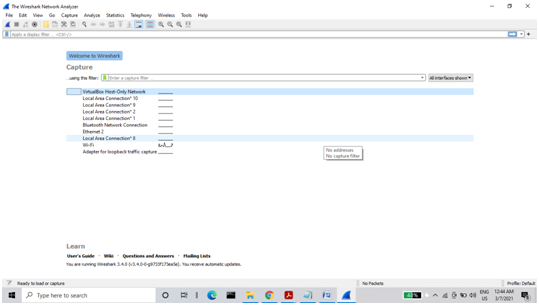
\includegraphics[width=5.56771in,height=3.13530in]{image6.png}\end{center}
  


\begin{quote}
The picture above shows the homescreen of version 3.4.0 of the
application.By selecting the current interface, we can get the traffic
traversing through that interface.
\end{quote}


\def\labelenumi{\arabic{enumi})}
\item
  The list in the above figure shows the Interface list options. That is
  the number of interfaces are present. The option that we select from
  the list will determine all the traffic we see. For instance, suppose
  we have selected the wi-fi option.the after this, a new window will
  open up, which shows the traffic that is flowing through the network
  currently. The picture below will show the live capture of packets
  from our wireshark.


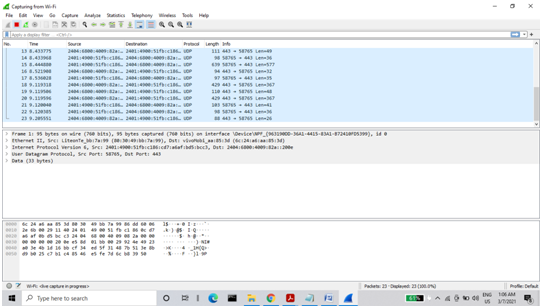
\includegraphics[width=5.60628in,height=3.16538in]{image3.png}


\def\labelenumi{\arabic{enumi})}
\item
  Now your analyzer is capturing packets that are flowing through your
  network and to analyze any packet, click on the red button in menu
  bar. The packet captured until yet is present in second part ``Packet
  listing window''.It determines the packet flow or the captured packets
  in the traffic. It includes the packet number, time, source,
  destination, protocol, length, and info.


\begin{quote}
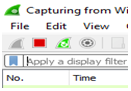
\includegraphics[width=1.30729in,height=0.89583in]{image4.png}

Below picture will show the list of captured packets

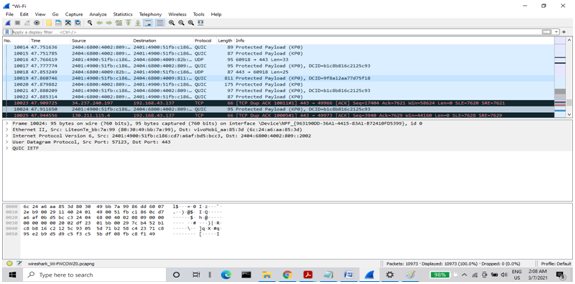
\includegraphics[width=5.60628in,height=3.16538in]{image1.png}
\end{quote}


\def\labelenumi{\arabic{enumi})}
\item
  There is a filter block below the menu bar, from where a large amount
  of data can be filtered. For example, if we apply a filter for HTTP,
  only the interfaces with the HTTP will be listed. If you want to
  filter according to the source, right-click on the source you want to
  filter and select 'Apply as Filter' and choose '...and filter.'
\end{enumerate}

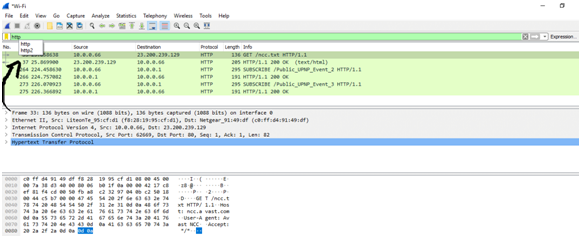
\includegraphics[width=5.60628in,height=3.16538in]{image2.png}

\chapter{\emph{Wireshark Packet Sniffing}}

It is a software that is mostly used by system administrators to isolate
and troubleshoot the problems over a network. It is also used by hackers
to analyze the packet of victims so that they can find any vulnerability
of the system and used it to exploit their victims. It can also be used
to capture any username and password that is transmitting without any
encrypted connection. The wrong way of its used is to drop user
confidential data.

Given below is the steps for packet sniffing over a network:

\begin{itemize}
\item
  Start your Wireshark Application.
\item
  Select the current interface. For example, the interface can be
  Ethernet that we would be using.
\item
  Now a continuous flow of traffic can be shown on our screen. To stop
  or watch any particular packet and want to analyze any packet, we can
  press the red button below the menu bar, it will stop capturing the
  packet and now we can analyze all the previously captured packets.
\end{itemize}

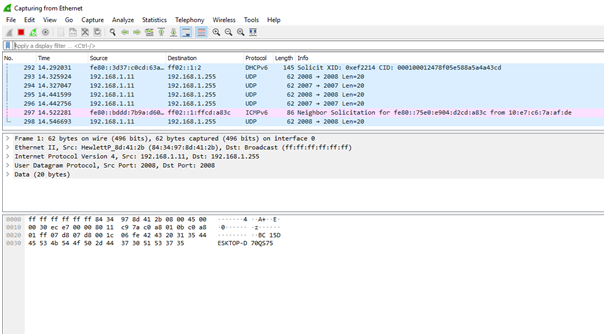
\includegraphics[width=6.26772in,height=3.45833in]{image7.png}
\\
Apply the filter by the name 'tcp.' After the filter is applied, the
screen will look as:
\\*

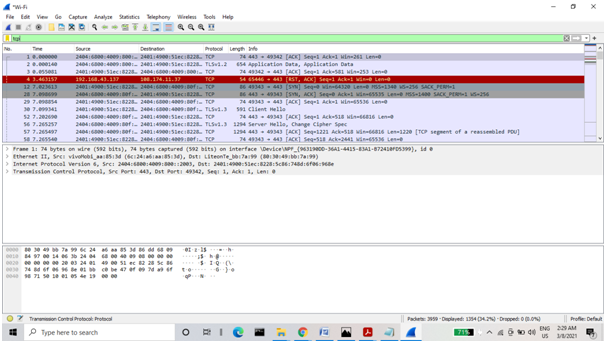
\includegraphics[width=6.26772in,height=3.52778in]{image8.png}
\\*
The above picture is showing all the traffic which follows `tcp'
protocol.

In the below picture we can see that it is capturing packets that are
flowing through this device,and wireshark is showing whole lots of
information about the packet.
\\*
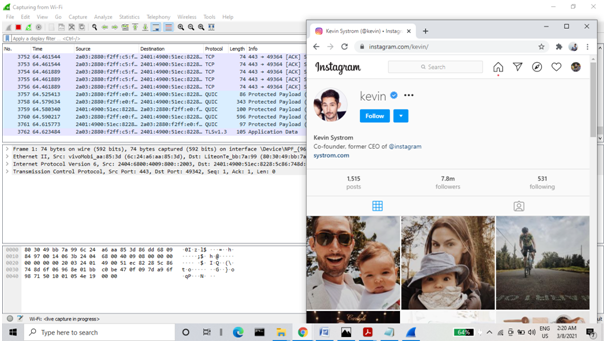
\includegraphics[width=6.26772in,height=3.52778in]{image10.png}
\\*
This process of capturing the packet and analyzing is called as ``Packet
Sniffing''.
\\*


\chapter{\emph{Implementation of tool that captures Network packets like
Wireshark} }

\subsection{Libraries required to capture the packets}

There are some specific libraries that are present in python library to
implement the process of capturing the packets that are flowing through
the network.

\begin{itemize}
\item
  Scapy
\end{itemize}

\begin{quote}
It is used for large scale web scraping, Scrapy is actually a python
framework. It provides us all the tools that we need to efficiently
\emph{\textbf{extract}} data from websites, and then process them as we
want, after that store them in the preferred \emph{\textbf{structure}}
and format.

As we all know the diverse nature of the internet, so there are no ``one
size fits all'' approach in extracting data from any of the websites.
Most of the time an ad hoc approach is taken and if we begin with
writing a code for every little task you perform, we would eventually
end up creating your own scraping framework. So there comes the Scrapy
framework.
\end{quote}

\begin{itemize}
\item
  Libpacp
\end{itemize}

\begin{quote}
libpcap is a lightweight Python package, based on the \emph{ctypes}
library.

It is fully compliant implementation of the original C \emph{libpcap}
from 1.0.0 up to 1.9.0 API and the \emph{WinPcap}'s 4.1.3 libpcap
(1.0.0rel0b) API by implementing whole its functionality in a clean
Python instead of C.
\end{quote}

\begin{itemize}
\item
  Libtrace
\end{itemize}

\begin{quote}
python-libtrace is not a complete set of all the libtrace routines,
rather it's a somewhat simplified set, intended as an easy-to-use
toolkit, and one that should be suitable for networking students. It use
(more or less) the original field names within the various header
decodes.
\end{quote}

\begin{itemize}
\item
  Socket Packet Capture
\end{itemize}

\begin{quote}
A simple packet sniffer in Python can be created with the help socket
module. We can use the raw

socket type to get the packets. A raw socket provides access to the
underlying protocols, which support

socket abstractions. Since raw sockets are part of the internet socket
API, they can only be used to

generate and receive IP packets.

The processing power used is comparatively lower than the existing
packet capturing libraries

\chapter{\emph{Methodology used for the preparation of Project }}
\end{quote}

\subsection{Methodology Used}

The Technique and Methodologies that we consider for the development for this project that is ``Network Packet Sniffer Tool Like Wireshark'' is rational unified process and evolutionary prototyping model. \\

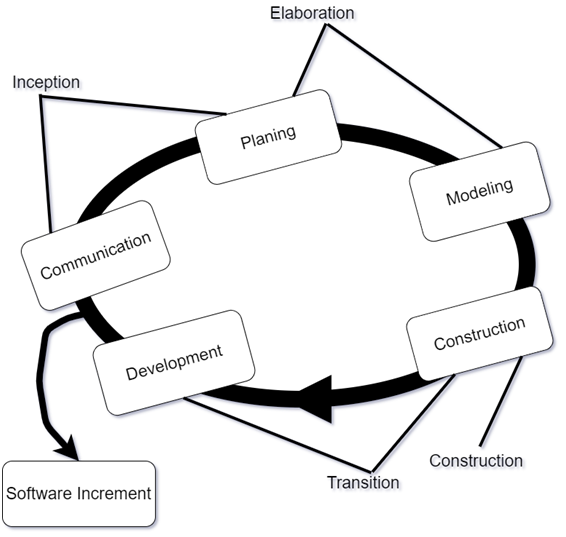
\includegraphics[width=4.85666in,height=3.55507in]{image9.png}

\emph{\large \textbf{Figure: Rational Unified process: Flow of the work\\}}

The Rational Unified Process is a kind of comprehensive process
framework that provides industry-tested practices for software and
systems delivery and implementation and for effective project
management. It is one of many processes contained within the Rational
Process Library.

Rational Unified Process recognizes the importance of customer
communication and streamlined methods for describing the customer's view
of a system. It suggests a process flow that is iterative and
incremental, providing the evolutionary feel that is essential in modern
software development (Pressman, 2010).


\subsection{ Software Dependencies:}

For the effective implementation/initialization of the project i.e.
Network sniffing with wireshark similar tool requires a proper execution
environment to be considered.

Python2.7 Programming Language accompanied with important libraries such
as STRUCT module, STRUCT module and JSON module.

For the proper implementation of our project, the most important
dependency of the project is the script has to be run with
administrative privileges.


\subsection{Hardware Dependencies:}


The major hardware dependencies contingent for the initialization of the
project are as follows:

\begin{itemize}
\item
  The System is dependent upon Mouse application.
\item
  The System is dependent upon Monitor application
\item
  Network Interface card is must for process of packet capture.
\item
  3-5 MB of hard disk space.
\item
  1 GB of RAM (Random Access Memory)
\end{itemize}
\newpage
\bigbreak
\subsection{\emph{References:}}
\begin{flushleft}
\href{https://www.javatpoint.com/wireshark}{\emph{https://www.javatpoint.com/wireshark}}
\bigbreak
\href{https://www.wireshark.org/docs/wsdg_html_chunked/PartDevelopment.html}{\emph{https://www.wireshark.org/docs/wsdg\_html\_chunked/PartDevelopment.html}}
\bigbreak
\href{https://www.analyticsvidhya.com/blog/2017/07/web-scraping-in-python-using-scrapy/\#:~:text=Scrapy\%20is\%20a\%20Python\%20framework,your\%20preferred\%20structure\%20and\%20format}{\emph{https://www.analyticsvidhya.com/blog/2017/07/web-scraping-in-python-using-scrapy/\#:~:text=Scrapy\%20is\%20a\%20Python\%20framework,your \ \%20preferred\%20structure\%20and\%20format}.}
\bigbreak
\href{https://pypi.org/project/libpcap/\#:~:text=libpcap\%20is\%20a\%20lightweight\%20Python,API\%20and\%20the\%20WinPcap's\%204.1}{\emph{https://pypi.org/project/libpcap/\#:~:text=libpcap\%20is\%20a\%20lightweight \ \%20Python,API\%20and\%20the\%20WinPcap's\%204.1}}
\end{flushleft}
\newpage
\chapter{Implementation of Packet Sniffer}

\section{Code for capturing packet  and store in a “.pcap” file:}
\emph{\large \textbf{Implemented by Abhilasha Sharma\\}}

\begin{lstlisting}[language=Python, style=chstyle]
        # Create socket 
        if os.name == "nt":
            conn = socket.socket(socket.AF_INET,socket.SOCK_RAW,socket.IPPROTO_IP)
            conn.bind((input("[+] YOUR_INTERFACE : "),0))
            conn.setsockopt(socket.IPPROTO_IP,socket.IP_HDRINCL,1)
            conn.ioctl(socket.SIO_RCVALL,socket.RCVALL_ON)
        else:
            conn = socket.socket(socket.AF_PACKET, socket.SOCK_RAW, socket.ntohs(0x0800))

        # datetime object containing current date and time

        #now = datetime.now()
        count=0

        rounds = int(input("\n\nEnter Number of Packets you want to capture: "))

        # dd/mm/YY H:M:S
        dt_string = time.strftime("%d-%m-%Y-%H:%M:%S")

        pcap_file1 = Pcap("Sniffed_packet_"+dt_string+".pcap")

        while True:
            
            count+=1

            raw_data, addr = conn.recvfrom(65535)
            
            pcap_file1.write(raw_data)



            dest_addr, src_addr, eth_proto, data = ethernet_frame(raw_data)
            print('\n Ehternet Frame: ')
            print(TAB_1 + 'Destination: {}, Source: {}, Protocol: {}'.format(dest_addr, src_addr, eth_proto))

 
            # 8 for IPv4

            if eth_proto ==8:
                (version, header_length, ttl, proto, src, target, data) = ipv4_packet(data)
                print(TAB_1 + 'IPv4_PAcket: ')
                print(TAB_2 + 'Version: {}, header_length: {}, TTL(Time to Live): {}'.format(version, header_length, ttl))
                print(TAB_2 + 'Protocol: {}, Source: {}, Target: {}'.format(proto, src, target))

             

                # 1 for ICMP

                if proto ==1:
                    (icmp_type, code, checksum, data) = ICMP_packet(data)
                    print(TAB_1 + 'ICMP_PAcket: ')
                    print(TAB_2 + 'Type: {}, Code: {}, Checksum: {}'.format(icmp_type, code, checksum))
                    print(TAB_2 + 'Data: {}')
                    print(format_multi_line(DATA_TAB_3, data))

  
                
                # 6 for TCP

                elif proto == 6:
                    (src_port, dest_port, sequence, acknowledgement, flag_urg, flag_ack, flag_psh, flag_rst, flag_syn, flag_fin, data) = tcp_packet(data)
                    print(TAB_1 + 'TCP Segment: ')
                    print(TAB_2 + 'Source port: {}, Destination port: {}'.format(src_port, dest_port))
                    print(TAB_2 + 'Sequence: {}, Acknowledgement: {}'.format(sequence, acknowledgement))
                    print(TAB_2 + 'Flags')
                    print(TAB_3 + 'URG: {}, ACK: {}, PSH: {}, RST: {}, SYN: {}, FIN: {}'.format(flag_urg, flag_ack, flag_psh, flag_rst, flag_syn, flag_fin))
                    print(TAB_2 + 'Data: {}')
                    print(format_multi_line(DATA_TAB_3, data))

 

                # 17 for UDP     

                elif proto == 17:
                    (src_port, dest_port, size, data) = udp_packet(data)
                    print(TAB_1 + 'UDP Segment: ')
                    print(TAB_2 + 'Source port: {}, Destination port: {}, Length: {}'.format(src_port, dest_port, size))
                    print(TAB_2 + 'Data: {}')
                    print(format_multi_line(DATA_TAB_3, data))

 
                # Other     

                else:
                    print(TAB_1 + 'Data: {}')
                    print(format_multi_line(DATA_TAB_2, data))

            else:
                print('Data: {}')
                print(format_multi_line(DATA_TAB_1, data))


 

            # flush data

            pcap_file1.pcap_file.flush()

            if count>=rounds:
                break

        # Closing the file
        pcap_file1.close()

\end{lstlisting}
\pagebreak
\section{Code for reading a “.pcap” file using scrapy:}
\emph{\large \textbf{Implemented by Ashish Sahu\\}}

\begin{lstlisting}[language=Python, style=chstyle]

       file_path = input("Enter your file name or file path: ")

        f_read = rdpcap(file_path)

        size1 = len(f_read)

        for packet in range(size1):

            pkt = f_read[packet]
            print(" Packet Information: \n\n")
            
            hexdump(pkt)

            print("\n\nFull Info of Packet: \n")
            pkt.show()


\end{lstlisting}

\section{Code for pcap class :}


\begin{lstlisting}[language=Python, style=chstyle]

PCAP_GLOBAL_HEADER_FMT = '@ I H H i I I I '


# Global Header Values
PCAP_MAGICAL_NUMBER = 2712847316
PCAP_MJ_VERN_NUMBER = 2
PCAP_MI_VERN_NUMBER = 4
PCAP_LOCAL_CORECTIN = 0
PCAP_ACCUR_TIMSTAMP = 0
PCAP_MAX_LENGTH_CAP = 65535
PCAP_DATA_LINK_TYPE = 1


class Pcap:

    def __init__(self, filename, link_type=PCAP_DATA_LINK_TYPE):
        self.pcap_file = open(filename, 'wb') 
        self.pcap_file.write(struct.pack('@ I H H i I I I ', PCAP_MAGICAL_NUMBER, PCAP_MJ_VERN_NUMBER, PCAP_MI_VERN_NUMBER, PCAP_LOCAL_CORECTIN, PCAP_ACCUR_TIMSTAMP, PCAP_MAX_LENGTH_CAP, link_type))
        print ("[+] Link Type : {}".format(link_type))




    def write(self, data):
        ts_sec, ts_usec = map(int, str(time.time()).split('.'))
        length = len(data)
        self.pcap_file.write(struct.pack('@ I I I I', ts_sec, ts_usec, length, length))
        self.pcap_file.write(data)

    def close(self):
        self.pcap_file.close()




\end{lstlisting}


\section{Code for Method used to show captured packets data at realtime:}
\emph{\large \textbf{Implemented by Abhijeet Singh\\}}

\begin{lstlisting}[language=Python, style=chstyle]

# Unpack Ethernet Frame

def ethernet_frame(data):
    src_mac, dest_mac, proto = struct.unpack("! 6s 6s H", data[:14])
    return get_mac_addr(dest_mac), get_mac_addr(src_mac), socket.htons(proto), data[14:]


# Return properly formatted MAC Address

def get_mac_addr(bytes_addr):
    bytes_str = map('{:02x}'.format, bytes_addr)
    return ':'.join(bytes_str).upper()


# Unpacking Ipv4 Packets

def ipv4_packet(data):
    version_header_length = data[0]
    version = version_header_length >> 4
    header_length = (version_header_length & 15) * 4
    ttl, proto, src, target = struct.unpack('! 8x B B 2x 4s 4s', data[:20])
    return version, header_length, ttl, proto, ipv4(src), ipv4(target), data[header_length:]


# Properly formatted Ipv4 address
    
#127.0.0.1

def ipv4(addr):
    return '.'.join(map(str, addr))


# Unpack ICMP PAckets

def ICMP_packet(data):
    icmp_type, code, checksum = struct.unpack('! B B H', data[:4])
    return icmp_type, code, checksum, data[4:]

# Unpack TCP Packet    

def tcp_packet(data):
    (src_port, dest_port, sequence, acknowledgement, offset_reserve_flags) = struct.unpack('! H H L L H', data[:14])
    offset = (offset_reserve_flags >> 12) * 4
    flag_urg = (offset_reserve_flags & 32) >> 5
    flag_ack = (offset_reserve_flags & 16) >> 4
    flag_psh = (offset_reserve_flags & 8) >> 3
    flag_rst = (offset_reserve_flags & 4) >> 2
    flag_syn = (offset_reserve_flags & 2) >> 1
    flag_fin = (offset_reserve_flags & 1)

    return src_port, dest_port, sequence, acknowledgement, flag_urg, flag_ack, flag_psh, flag_rst, flag_syn, flag_fin, data[offset :]


# Unpack UDP PAcket

def udp_packet(data):
    src_port, dest_port, size = struct.unpack('! H H 2x H', data[:8])
    return src_port, dest_port, size, data[8:]



# formats multi line data

def format_multi_line(prefix, string, size = 80):
    size -= len(prefix)
    if isinstance(string, bytes):
        string = ''.join(r'\x{:02x}'.format(byte) for byte in string)
        if size % 2:
            size -=1

    return '\n'.join([prefix + line for line in textwrap.wrap(string, size)])



\end{lstlisting}



\subsection{Contribution of each member towards Project:}

\subsubsection{Member 1: Abhilasha Sharma}
\begin{enumerate}
    \item Writing documents :
        \begin{itemize}
        \item   Project Purpose
        \item   Basic definitions of  relevant topics that includes
                \begin{itemize}
                        \item Introduction to sniffing
                        \item What is packet sniffing
                        \item Tools used for packet sniffing
                        \item What is wireshark and use of wireshark
                \end{itemize}		
        \item   Reference of websites

    \end{itemize}
    
    \item Creating PPT
        \begin{itemize}
            \item Introduction to project 
            \item    	Basic purpose of the project 
            \item    	Brief introduction to sniffing
            \item    	What are packet sniffers
            \item    	Tools that are being used for packet sniffing
	        \item            Wireshark and its usage
        \end{itemize}
    
    \item Contribution in creating the project:

        \begin{itemize}
            \item Creating a pcap file when a new session for packet capture is created
        	\item Using socket to create connection
        	\item After capturing packet using Pcap class to store packet info
        	\item Showing real-time basic information of captured packet
        \end{itemize}
\end{enumerate}



\subsubsection{Member 2: Ashish Sahu}
\begin{enumerate}
    \item Writing documents :
        \begin{itemize}
        \item   Wireshark Demonstration
    	\item Working of Wireshark
    	\item Choosing an interface to capture packet
    	\item Start capturing 
        \item How wireshark captures packets
        \item How to analyze different packets(TCP, UDP,ICMP, DNS, etc) in wireshark 

    \end{itemize}
    
    \item Creating PPT
        \begin{itemize}
            \item Demonstration of Wireshark
        	\item Steps to capture packets in wireshark
        	\item How to read pcap files in wireshark
        	\item Analyze packets using a set of tools available in wireshark to gain information.

        \end{itemize}
    
    \item Contribution in creating the project:

        \begin{itemize}
            \item Creating a Class “Pcap” that will take captured packet as input and store it in a “.pcap” file
            \item Reading a “.pcap” from a given path
            \item Printing all the information of packet captured

        \end{itemize}
\end{enumerate}

\subsubsection{Member 3: Abhijeet Singh}
\begin{enumerate}
    \item Writing documents :
        \begin{itemize}
            \item Description of packages that are used in project:
		    \begin{itemize}
		        \item Scapy
        		\item Socket
        		\item Textwrap
        		\item Struct
		    \end{itemize}
        	\item Purpose of each package
        	\item Methodology used for creating project
        	\item References

    \end{itemize}
    
    \item Creating PPT
        \begin{itemize}
            \item Packages used for working of the project
        	\item Brief description of each package any their functioning
        	\item Scrapy, textwrap, struct, socket, etc
        	\item Methodology used for creating the project 
        
        \end{itemize}
    
    \item Contribution in creating the project:

        \begin{itemize}
            \item Packages that are required for working of project
	\item Writing methods for showing real-time description on each captured packet
	\item Ex: icmp-segment, tcp-segment,udp-segment etc methods
	\item Designing basic structure of packet sniffer 
	\item Adding comments at the required places


        \end{itemize}
\end{enumerate}

\pagebreak

\subsection{\Large \emph{References: }}
\begin{flushleft}
\href{https://medium.com/@vworri/extracting-the-payload-from-a-pcap-file-using-python-d938d7622d71}{\emph{https://medium.com/@vworri/extracting-the-payload-from-a-pcap-file-using-python-d938d7622d71}}
\bigbreak
\href {https://subscription.packtpub.com/book/networking_and_servers/9781784399771/8/ch08lvl1sec48/reading-and-writing-to-pcap-files}{\emph{https://subscription.packtpub.com/book/networking_and_servers/9781784399771/8/ch08lvl1sec48/\linebreak reading-and-writing-to-pcap-files}}
\bigbreak
\href {https://cppsecrets.com/users/812115971219710810510797110971151014957494864103109971051084699111109/Python-Scapy-Reading-PCAP-file.php}{\emph{https://cppsecrets.com/users/\linebreak 812115971219710810510797110971151014957494864103109971051084699111109/Python-Scapy-Reading-PCAP-file.php}}
\bigbreak
\href {https://youtu.be/WGJC5vT5YJo}{\emph{https://youtu.be/WGJC5vT5YJo}}
\bigbreak
\href {https://www.bitforestinfo.com/blog/01/13/save-python-raw-tcpip-packet-into-pcap-files.html}{\emph{https://www.bitforestinfo.com/blog/01/13/save-python-raw-tcpip-packet-into-pcap-files.html}}
\bigbreak
\href {https://stackoverflow.com/questions/18256342/parsing-a-pcap-file-in-python}{\emph{https://stackoverflow.com/questions/18256342/parsing-a-pcap-file-in-python}}
\bigbreak
\href {https://patorjk.com/software/taag/#p=display&f=Georgia11&t=Sniffer%20/ } {\emph{https://patorjk.com/software/taag/#p=display&f=Georgia11&t=Sniffer%20/}}
\bigbreak
\href {https://fsymbols.com/generators/carty/} {\emph{https://fsymbols.com/generators/carty/}}
\bigbreak
\href {https://www.colorschemer.com/ascii-art-generator/#p=display&f=Avatar&t=Sniffer}{\emph{https://www.colorschemer.com/ascii-art-generator/#p=display&f=Avatar&t=Sniffer}}
\end{flushleft}

\chapter{Output of Project}

\subsection{Screenshot of running processes}

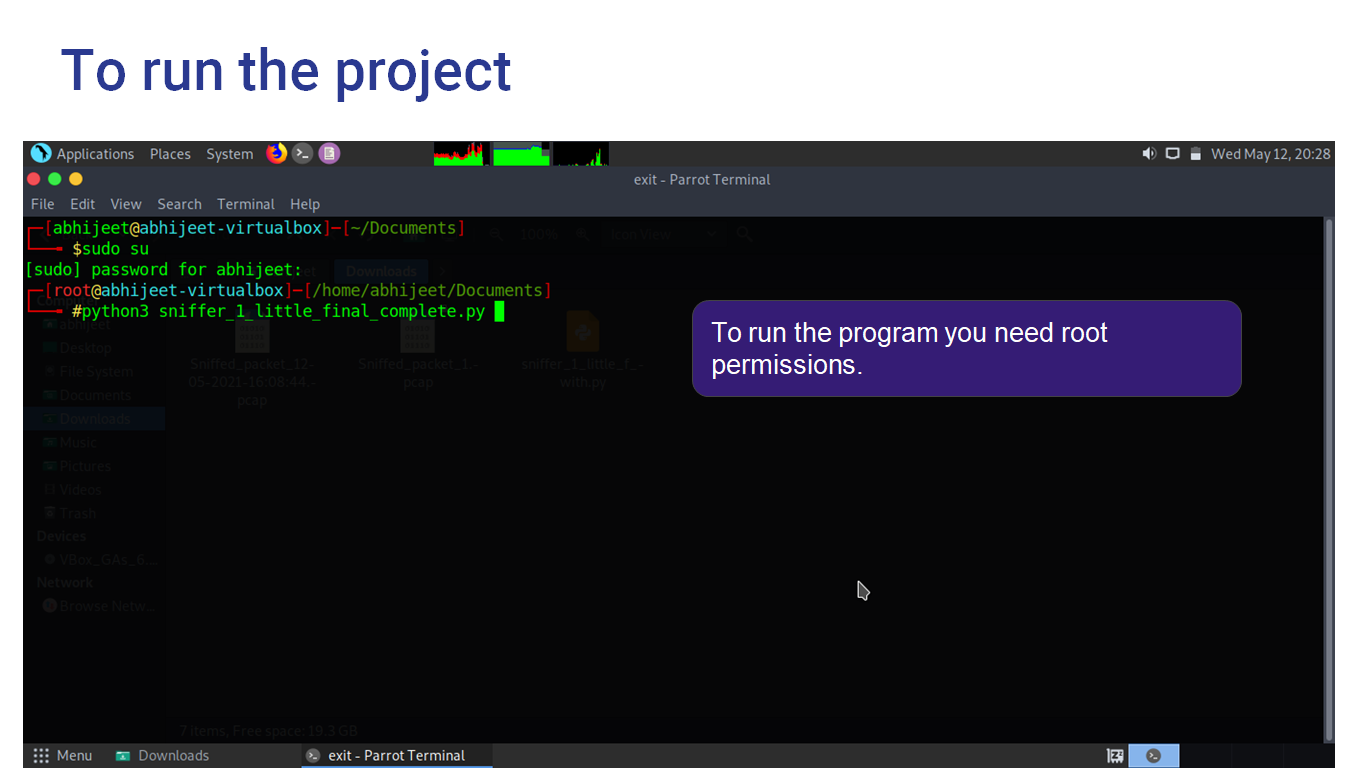
\includegraphics[width=6.85666in,height=3.55507in]{Screenshot (10).png}

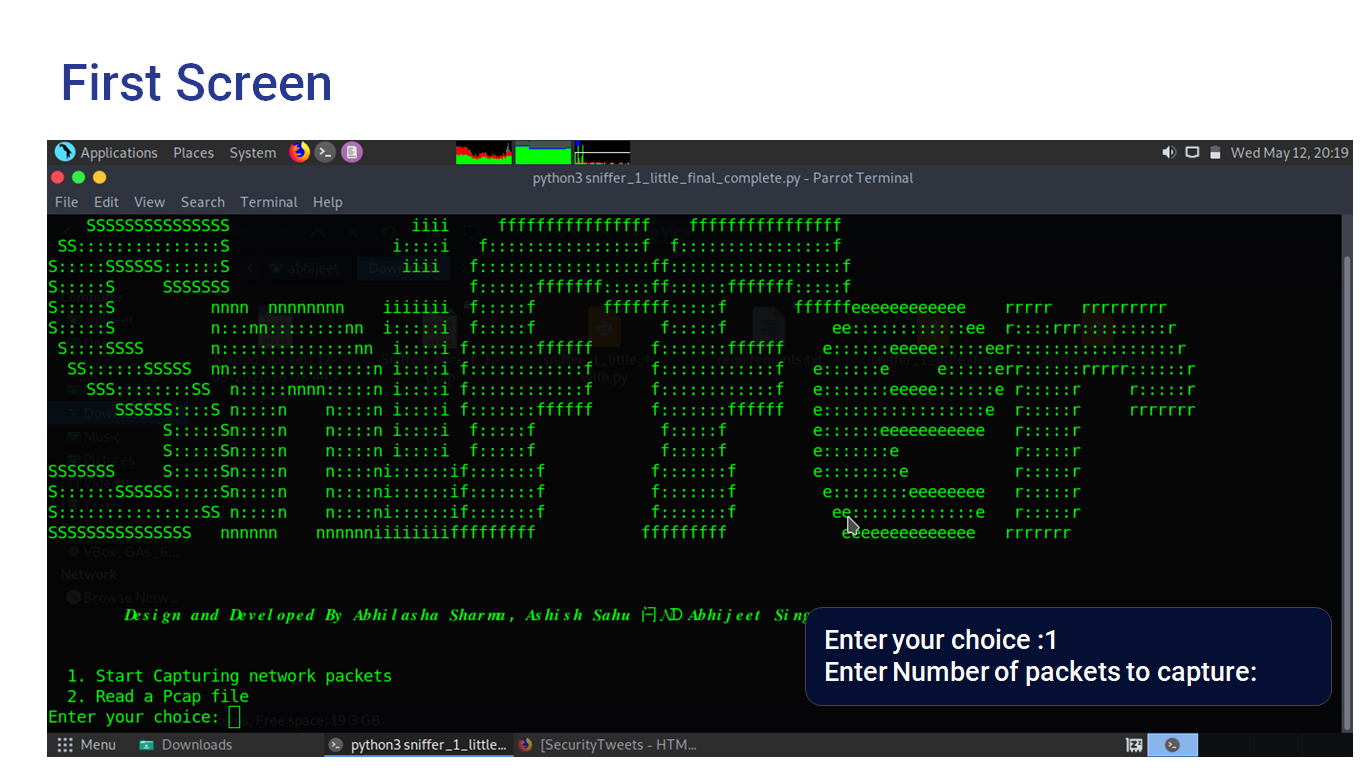
\includegraphics[width=6.85666in,height=3.55507in]{Screenshot (11).png}

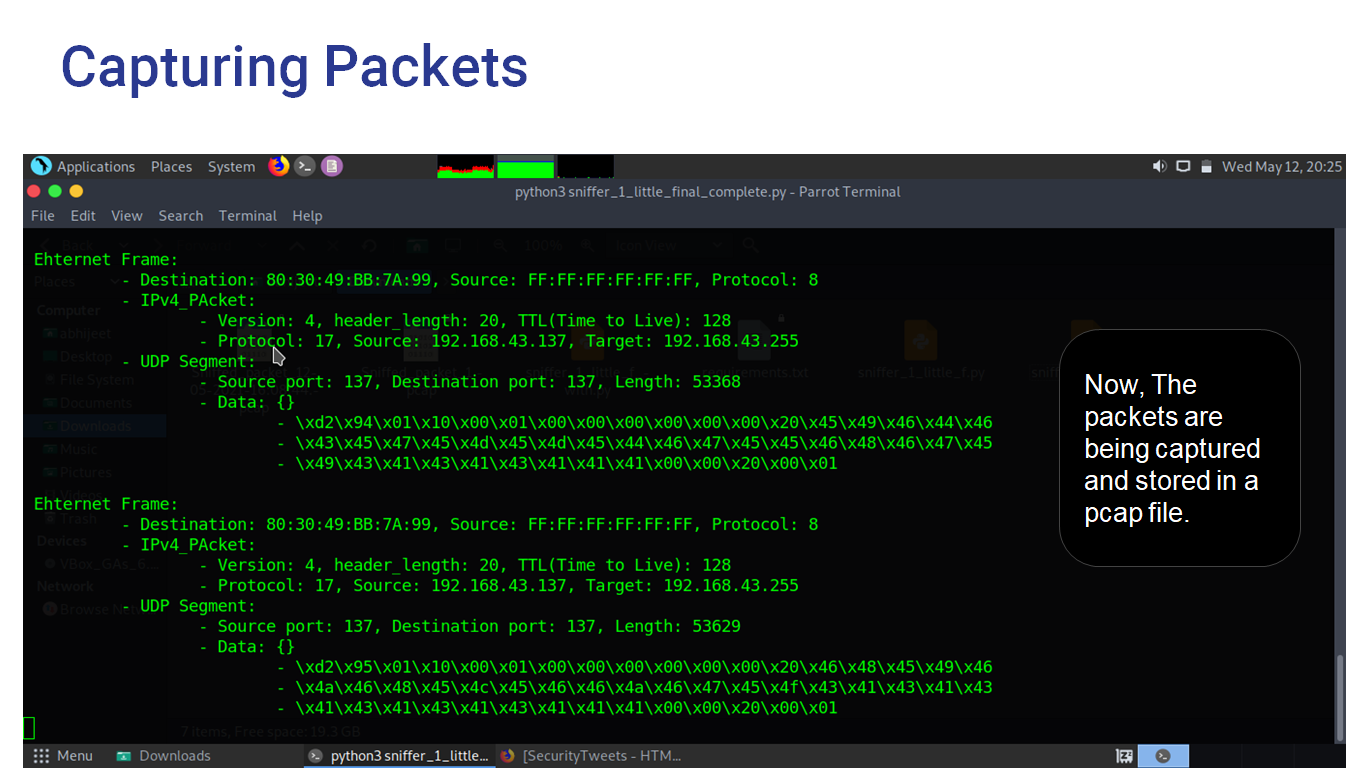
\includegraphics[width=6.85666in,height=3.55507in]{Screenshot (12).png}

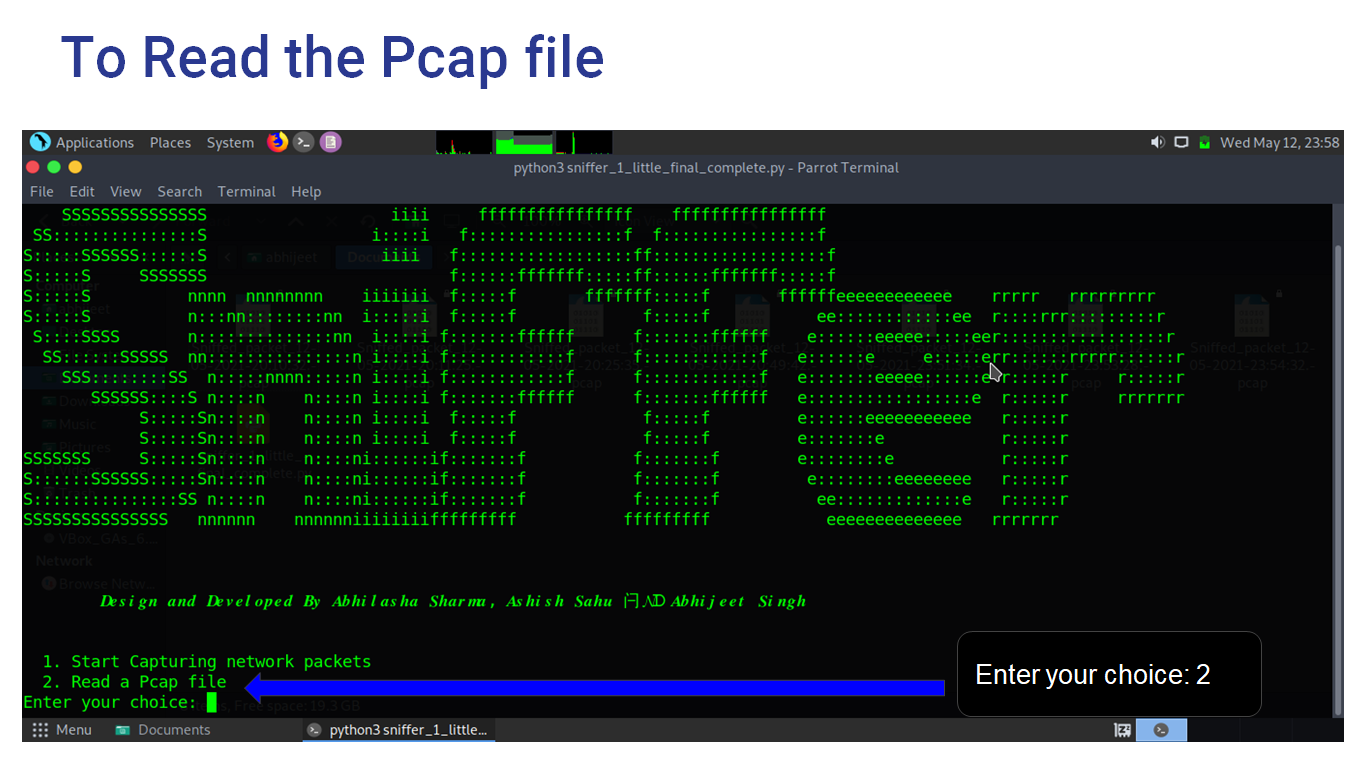
\includegraphics[width=6.85666in,height=3.55507in]{Screenshot (13).png}

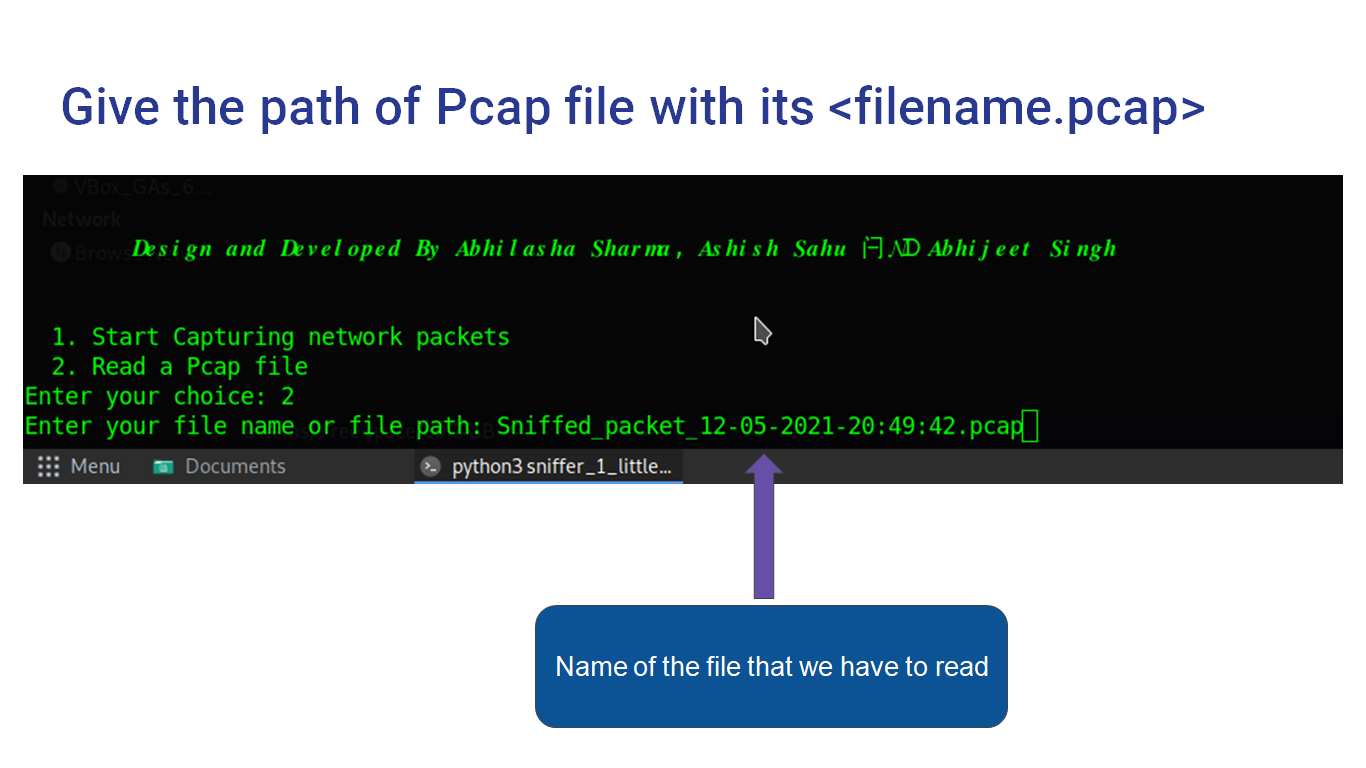
\includegraphics[width=6.85666in,height=3.55507in]{Screenshot (14).png}

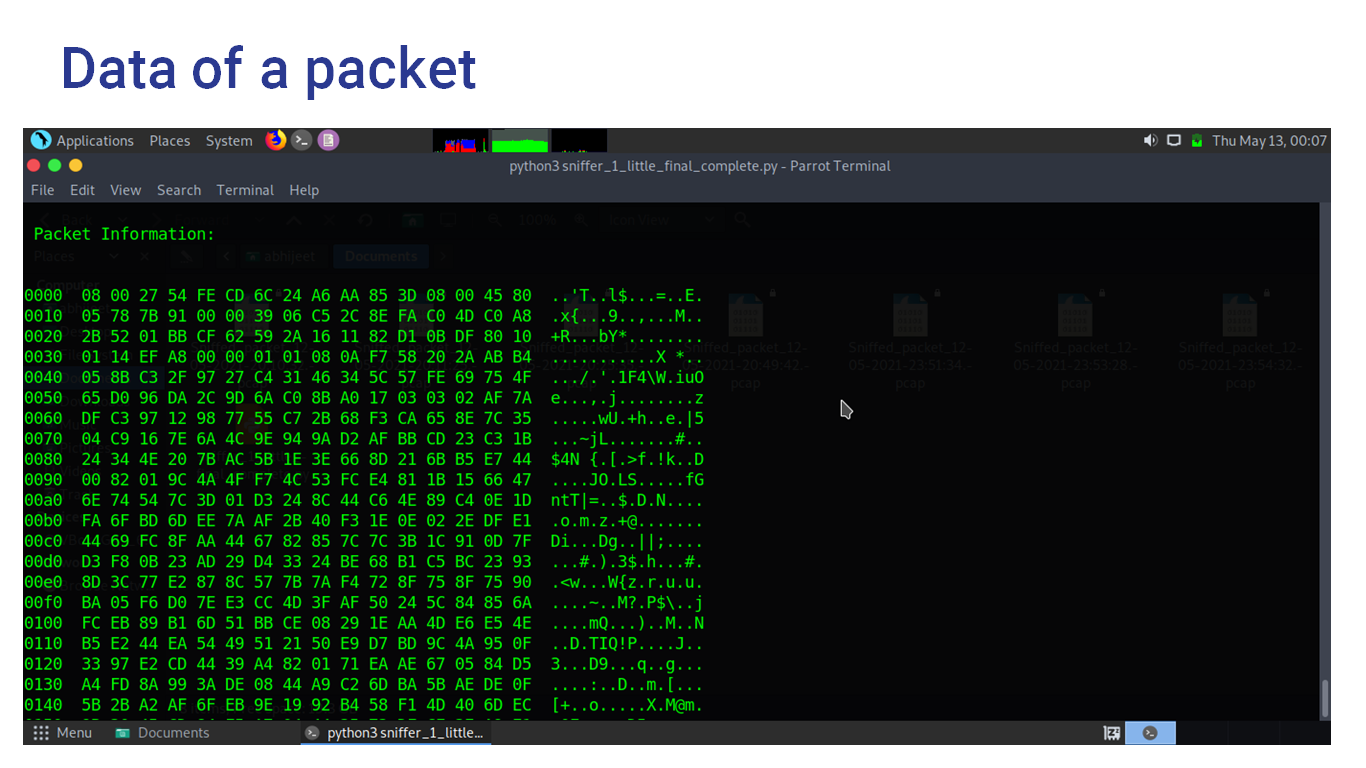
\includegraphics[width=6.85666in,height=3.55507in]{Screenshot (15).png}

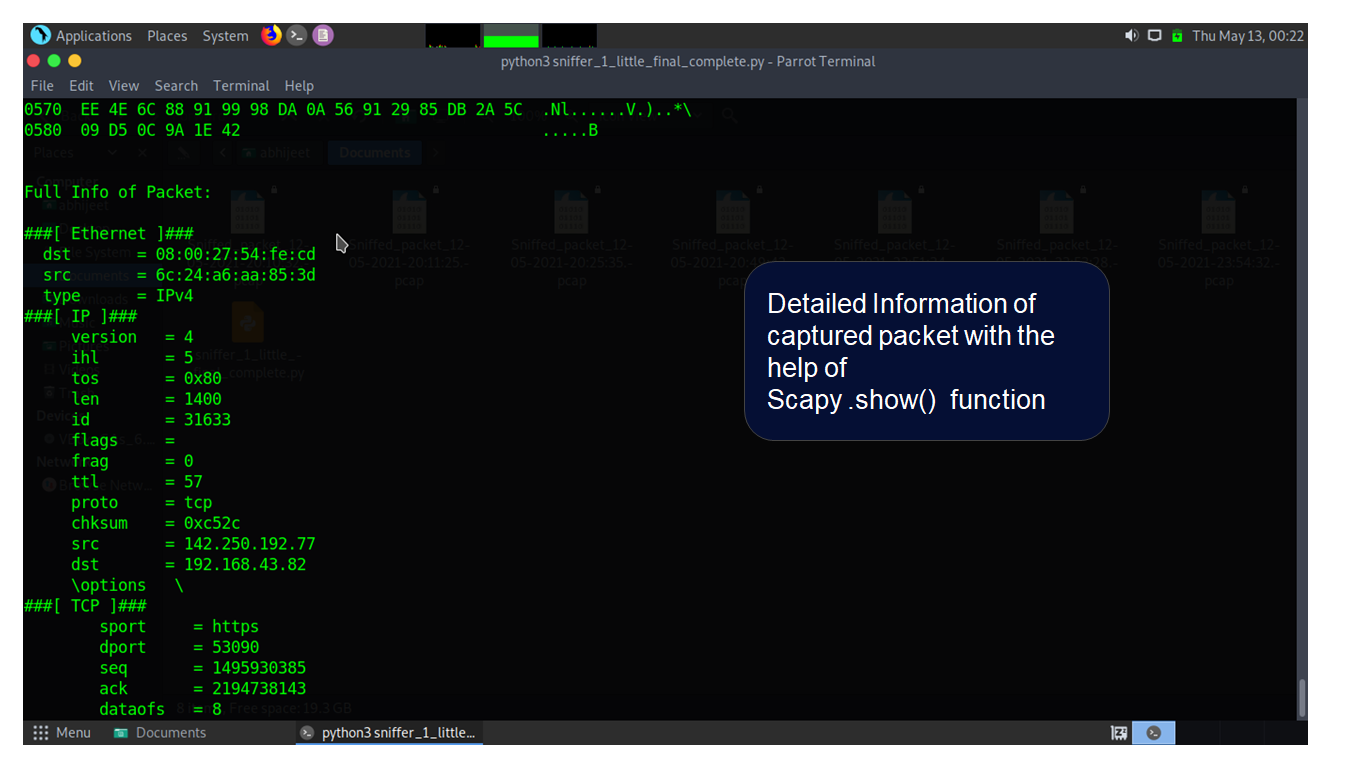
\includegraphics[width=6.85666in,height=3.55507in]{Screenshot (16).png}

\pagebreak

    

\begin{flushleft}

\textbf{\LARGE \bf \emph{\begin{center}
    Conclusion:
\end{center}}}
\end{flushleft}

\paragraph{The most important purpose of this project is to develop a nifty tool(
or a software) that have the ability to sniff over the network and
capture data packets that is around it. Analyze those packets and gain
some informative data from it to compromise the systems on its range. It
can also be used to monitor a user's home network for activities that
are being encapsulated in the process.There are many expensive tools out
there for this purpose but it won't fits on an average students pocket
money, so to help those people who really wants to know what is going on
with their home network this project can be name ``Network Sniffing With
Wireshark Similar Tool''. It would turn out to be a great help and
guidance. From the current scenarios of this highly tempting and cunning
world this tool come on the light that not just feasible for monitoring
the network but can be used effective in the field of education as well.}



\end{document}


